\documentclass[10pt,a4paper]{article}
\usepackage[top=19mm,bottom=25.4mm,left=16mm,right=16mm]{geometry}
\usepackage{fontspec,graphicx,amsmath,amssymb,multicol,booktabs,array,tabularx}
\usepackage[hidelinks]{hyperref}
\setmainfont{Times New Roman}
\setlength{\columnsep}{6mm}
\setlength{\parindent}{0pt}
\setlength{\parskip}{3pt}
\setlength{\multicolsep}{4pt}
\setlength{\abovedisplayskip}{4pt}
\setlength{\belowdisplayskip}{4pt}
\pagestyle{empty}
\makeatletter
\renewcommand{\section}{\@startsection{section}{1}{0pt}{5pt}{2pt}{\normalfont\normalsize\bfseries}}
\makeatother
\newcommand{\sect}[1]{\section*{#1}}
\begin{document}
\begin{center}
\includegraphics[width=\textwidth]{baic2026_header.png}\par\vspace{4pt}
{\fontsize{14}{17}\selectfont\bfseries Hard-Budget Feature Selection with Resampled Mutual-Information Repair in EHOA}\par
Amirreza Ghaffarian\par
Graduate Student, Islamic Azad University\end{center}
\textbf{Abstract. } We evaluate four hard-budget repairs within EHOA using a redesigned training pipeline. Mutual-information utility is fitted only on the training rows of each inner fold, and candidate repair, imputation, scaling and SMOTE use only that fold and its selected dimensions. The final mask uses outer-training utility; outer test data never enter selection. We complete 774 fresh runs: 450 primary runs on ten datasets and 324 sensitivity runs on three biomedical datasets. Steel uses 27 predictors and seven classes, while Parkinson recordings use subject-prefix-disjoint folds. At a 30\% synthetic budget, resampled repair attains mean balanced accuracy 0.7943, cost ratio 0.2768 and Nogueira stability 0.2216. Friedman balanced-accuracy p is 0.09455. Pairwise effects, Holm corrections and descriptive dataset-bootstrap intervals qualify the conclusions. Sensitivity covers budgets, resample counts and utility penalties. All constrained final masks satisfy their budgets. The study evaluates an acquisition-constrained computational procedure with synthetic costs; it does not establish clinical validity or universal superiority. The protocol was frozen locally before execution, with prior archived findings already known.

\textbf{Keywords. } feature selection, hard budget, resampled mutual information, subset stability
\begin{multicols}{2}\raggedcolumns
\sect{1  Problem and contribution}
A small feature set need not be inexpensive: acquisition costs can differ between variables. Hard-budget selection limits the sum of selected costs [1]. Subset stability measures how feature choices vary across training samples and random search, rather than how accuracy or convergence varies [2]. In biomedical classification, this distinction matters when investigators interpret a selected measurement panel.

Medical feature selection spans imaging, signals and molecular data [3]. Predictive discrimination, reproducible feature identity and acquisition burden are separate objectives. Correlated descriptors can substitute for one another, so a changing mask need not imply poor prediction; conversely, a repeated mask does not establish a valid biomarker. This motivates reporting balanced accuracy, cost and chance-corrected subset stability together.

We retain the EHOA search [4] and compare unconstrained EHOA with four repairs using the same selected-dimension evaluation pipeline. Among constrained variants, only repair utility differs. FoldSafeEHOA implements fold-local utility and candidate-specific training; these fresh results are separate from the archived CostStableEHOA protocol. The contribution is a controlled, auditable comparison, not a new optimization family.

\sect{2  Related studies}
Stability metrics can reward reproducible yet weak predictors; importance-weighted stability addresses this concern [5]. Medical budget selection with penalized risk [6], sequential acquisition [7], and grouped costs with shadow features [8] solve related but different problems. Table 1 summarizes these distinctions; NR means not reported in the inspected source. Their numerical results are not directly comparable with our protocol.

\par\vspace{3pt}\begin{minipage}{\linewidth}{\footnotesize Table 1. Related-work comparison. Full evaluation details are in the supplement.\par}
{\fontsize{6.8}{8.3}\selectfont\setlength{\tabcolsep}{2pt}\renewcommand{\arraystretch}{1.1}
\begin{tabularx}{\linewidth}{>{\hsize=1.0000\hsize\raggedright\arraybackslash}X>{\hsize=1.0000\hsize\raggedright\arraybackslash}X>{\hsize=1.0000\hsize\raggedright\arraybackslash}X>{\hsize=1.0000\hsize\raggedright\arraybackslash}X>{\hsize=1.0000\hsize\raggedright\arraybackslash}X>{\hsize=1.0000\hsize\raggedright\arraybackslash}X}\toprule
Study & Budget & Costs & Stability & Evaluation & Difference\\\midrule
Jagdhuber [1] & Yes & Additive & NR & Simulation & Feasible GA\\
Nogueira [2] & NR & NR & Chance-corrected & Resampling & Metric\\
Hamer [5] & NR & NR & Importance-weighted & Resampling & Metric limits\\
Klonecki [6] & Yes & Feature / proxy & NR & Medical data & Penalized ERM\\
Valancius [7] & NR & Sequential & NR & AFA benchmarks & Patient-wise policy\\
Klonecki [8] & Yes & Grouped & NR & MIMIC & Shadow stopping\\
This work & Yes & Synthetic additive & Nogueira & 3 x 3 outer & MI/cost repair\\
\bottomrule\end{tabularx}}
\end{minipage}\par\vspace{3pt}
Classical stability selection aggregates repeated subsample selections and, under specified assumptions and thresholds, controls false selections [9,10]. Our four MI resamples instead estimate a deletion utility before wrapper search. We neither threshold repeated selection probabilities nor inherit those error-control guarantees. Nogueira stability evaluates the final masks [2]; it is not the optimized fitness. Active acquisition [7] chooses measurements sequentially per case, whereas our repair returns a fixed feasible subset.

\sect{3  Implemented EHOA}
Each hiker has a continuous position x and a velocity v; a binary mask z selects features. Initialization uses a tent sequence with initial value 0.7 and parameter 0.4, mapped to [-6,6]. Velocities start uniformly in [-1.2,1.2]. For iteration t of T=10, the implemented update is:

\begin{equation}\begin{gathered}\begin{aligned}v_i\leftarrow\operatorname{clip}_{[-12,12]}\big(&w_t v_i+SF_t[2r_1(p_i-x_i)\\&+2r_2(g-x_i)]\big)\end{aligned}\end{gathered}\end{equation}
\begin{equation}\begin{gathered}\begin{gathered}x_i\leftarrow\operatorname{clip}_{[-6,6]}(x_i+v_i)\\w_t=0.9-0.5t/T,\quad SF_t=3-2t/T\end{gathered}\end{gathered}\end{equation}
Here p\_i and g are personal and global best continuous positions, and r\_1,r\_2 are independent per-feature uniform draws. The sigmoid gives selection probability 1/(1+exp(-x\_j)); an empty sampled mask restores the largest probability. The implementation keeps continuous leaders separate from repaired masks, caches fitness for duplicate masks, and stops after ten iterations without early stopping.

\sect{4  Fold-local budget repair and stability}
Costs are fixed positive synthetic additive units, drawn with NumPy seed 1000+D from lognormal(0,0.7). The primary budget is B=0.30 sum(c); sensitivity uses 0.15 and 0.50. Costs are independent of labels and do not represent money. Every constrained nonempty mask must satisfy sum(z\_j c\_j)<=B. Shared acquisition costs require a different grouped model [6,8].

\begin{equation}\begin{gathered}u_j=\max(0,\overline I_j-\lambda s_j),\quad q_j=u_j/c_j\end{gathered}\end{equation}
For each inner fold, MI is fitted to its imputed training rows only. Four class-stratified samples draw ceil(0.8 n\_class) rows with replacement (minimum two). The continuous-discrete estimator uses three neighbors [11]; Dermatology treats its first 33 categorical/ordinal inputs as discrete and age as continuous. MI is in nats and s\_j is sample SD. Lambda=1 gives a conservative utility, not a calibrated confidence bound; there is no division by sqrt(R). Final outer-training utility is separate and never used to repair inner-validation candidates.

\par\vspace{3pt}\begin{minipage}{\linewidth}{\footnotesize Table 2. Four repairs share the same deletion rule.\par}
{\fontsize{6.8}{8.3}\selectfont\setlength{\tabcolsep}{2pt}\renewcommand{\arraystretch}{1.1}
\begin{tabularx}{\linewidth}{>{\hsize=1.0000\hsize\raggedright\arraybackslash}X>{\hsize=1.0000\hsize\raggedright\arraybackslash}X>{\hsize=1.0000\hsize\raggedright\arraybackslash}X}\toprule
Repair & Utility u\_j & Meaning\\\midrule
Random/cost & U(0,1), fixed per training fold & Not uniform deletion\\
Cheapest & 1 & Largest cost first\\
MI/cost & Single-sample MI & Relevance per cost\\
Resampled/cost & max(0, mean MI - SD) & Conservative heuristic\\
\bottomrule\end{tabularx}}
\end{minipage}\par\vspace{3pt}
Search samples a raw mask. Each inner fold repairs this candidate with its own training utility, then fits imputation, scaling and SMOTE on the selected columns [12]. Validation rows are only transformed and predicted. Fitness averages ordinary accuracy and selected size across three independently repaired folds. The winning raw candidate is finally repaired with outer-training utility; inner and final masks may differ. The outer classifier is refitted using only final selected columns. This evaluates a complete selection-and-repair procedure, not a fixed mask reused across all inner folds [13].

\begin{equation}\begin{gathered}\begin{gathered}F(z)=\frac13\sum_{f=1}^3F_f(z)\\F_f(z)=0.99(1-Acc_f)+0.01k_f/D\end{gathered}\end{gathered}\end{equation}
Deletion removes the active feature minimizing utility/cost while over budget. An unaffordable singleton is cleared; an empty mask restores the affordable highest-ratio feature. Positive costs and finite deletion ensure feasibility when one feature is affordable, as verified here. This guarantees budget compliance, not optimal prediction. MI remains marginal and can overlook interactions or redundancy.

\begin{equation}\begin{gathered}\Phi=\operatorname{clip}_{[-1,1]}\left(1-\frac{\frac M{M-1}\frac1D\sum_j p_j(1-p_j)}{(\bar k/D)(1-\bar k/D)}\right)\end{gathered}\end{equation}
Nogueira stability [2] uses M=9 final masks per dataset/configuration, selection frequencies p\_j and mean size k-bar. Identical full/empty masks return one in the code. The masks overlap in training data and are dependent; their copied stability values are not nine independent observations. Jaccard is a supplementary, uncorrected overlap measure.

\sect{5  Datasets and source corrections}
\par\vspace{3pt}\begin{minipage}{\linewidth}{\footnotesize Table 3. Fresh-run dataset specifications; U links to archive.ics.uci.edu/dataset/\{id\}.\par}
{\fontsize{6.8}{8.3}\selectfont\setlength{\tabcolsep}{2pt}\renewcommand{\arraystretch}{1.1}
\begin{tabularx}{\linewidth}{>{\hsize=1.8947\hsize\raggedright\arraybackslash}X>{\hsize=0.5684\hsize\raggedright\arraybackslash}X>{\hsize=0.3789\hsize\raggedright\arraybackslash}X>{\hsize=0.3789\hsize\raggedright\arraybackslash}X>{\hsize=2.1474\hsize\raggedright\arraybackslash}X>{\hsize=0.6316\hsize\raggedright\arraybackslash}X}\toprule
Dataset & N & D & K & Class counts & Source\\\midrule
Breast Cancer & 569 & 30 & 2 & 212/ 357 & U17\\
Wine & 178 & 13 & 3 & 59/ 71/ 48 & U109\\
Ionosphere & 350 & 34 & 2 & 125/ 225 & U52\\
Sonar & 208 & 60 & 2 & 111/ 97 & U151\\
Dermatology & 366 & 34 & 6 & 112/ 61/ 72/ 49/ 52/ 20 & U33\\
Spambase & 4210 & 57 & 2 & 2531/ 1679 & U94\\
Parkinson (grouped) & 195 & 22 & 2 & 48/ 147 & U174\\
Hill Valley & 1212 & 100 & 2 & 606/ 606 & U147\\
Steel (corrected) & 1941 & 27 & 7 & 158/ 190/ 391/ 72/ 55/ 402/ 673 & U198\\
Madelon & 2600 & 500 & 2 & 1300/ 1300 & U171\\
\bottomrule\end{tabularx}}
\end{minipage}\par\vspace{3pt}
Exact (X,y) duplicates are removed: Ionosphere uses 350 rows and Spambase 4210. Steel removes six target-indicator inputs and reconstructs seven fault classes. Parkinson recordings match the UCI numeric file and use 32 subject prefixes in both outer and inner group splits. The UCI narrative states 31 participants, so clinical group identity remains unverified. Original raw data and earlier results are preserved.

\sect{6  Fresh protocol and statistical analysis}
The local protocol and code hashes were frozen before execution, after earlier archived results were known. This is a new exploratory study, not independent public preregistration. Three seeds and three outer folds yield 450 primary runs across ten datasets and five methods. We additionally complete 324 prespecified sensitivity runs on Breast Cancer, Dermatology and Parkinson. All methods share splits, cost vectors, search size and candidate-specific preprocessing. Inner utility uses training labels only; inner fitness remains an optimized selection score. Outer tests provide performance estimates.

\par\vspace{3pt}\begin{minipage}{\linewidth}{\footnotesize Table 4. Actual frozen settings.\par}
{\fontsize{6.8}{8.3}\selectfont\setlength{\tabcolsep}{2pt}\renewcommand{\arraystretch}{1.1}
\begin{tabularx}{\linewidth}{>{\hsize=1.0000\hsize\raggedright\arraybackslash}X>{\hsize=1.0000\hsize\raggedright\arraybackslash}X}\toprule
Parameter & Value\\\midrule
Population / iterations & 8 / 10; no early stop\\
Position / velocity clip & [-6,6] / [-12,12]\\
Tent / sweep / inertia & 0.7,p=0.4 / 3 to 1 / 0.9 to 0.4\\
c1,c2 / alpha & 2,2 / 0.99\\
Outer / inner folds & 3 / 3; Parkinson grouped\\
Outer seeds & 72001,72002,72003\\
Selector seed & outer seed + fold index x 100003\\
Primary R / fraction / lambda & 4 / 0.8 with replacement / 1\\
Sensitivity R / lambda & 4,8,16 / 0,1,2; OFAT\\
Cost / budgets & lognormal(0,0.7) / 15,30,50\%\\
Classifier & 5-NN; uniform; Euclidean\\
Imputation / scale / SMOTE & Training-selected columns only\\
Timing & Includes utility and final classification\\
\bottomrule\end{tabularx}}
\end{minipage}\par\vspace{3pt}
Each dataset supplies one mean per method and one stability estimate [14]. Friedman tests use ten dataset blocks, tie correction and df=4. Two-sided Wilcoxon compares resampled repair with four controls, followed by Holm within each metric and across all 24 contrasts. Six omnibus tests are also corrected. Dataset-bootstrap intervals use 20,000 draws (seed 20261012) and are descriptive and unadjusted. Nine overlapping folds are never treated as independent replicates.

\sect{7  Results and sensitivity}
\par\vspace{3pt}\begin{minipage}{\linewidth}{\footnotesize Table 5. Equal-weight means over ten datasets; V is budget exceedance.\par}
{\fontsize{6.8}{8.3}\selectfont\setlength{\tabcolsep}{2pt}\renewcommand{\arraystretch}{1.1}
\begin{tabularx}{\linewidth}{>{\hsize=1.0000\hsize\raggedright\arraybackslash}X>{\hsize=1.0000\hsize\raggedright\arraybackslash}X>{\hsize=1.0000\hsize\raggedright\arraybackslash}X>{\hsize=1.0000\hsize\raggedright\arraybackslash}X>{\hsize=1.0000\hsize\raggedright\arraybackslash}X>{\hsize=1.0000\hsize\raggedright\arraybackslash}X}\toprule
Method & BA & Cost ratio & Size & Stability & V\\\midrule
EHOA & 0.7931 & 0.4923 & 42.70 & 0.1183 & 88/90\\
Random/cost & 0.7794 & 0.2717 & 31.43 & 0.1160 & 0/90\\
Cheapest & 0.7961 & 0.2758 & 34.90 & 0.2861 & 0/90\\
MI/cost & 0.7961 & 0.2773 & 27.28 & 0.2250 & 0/90\\
Resamp./cost & 0.7943 & 0.2768 & 31.31 & 0.2216 & 0/90\\
\bottomrule\end{tabularx}}
\end{minipage}\par\vspace{3pt}
\par\vspace{3pt}\begin{minipage}{\linewidth}{\footnotesize Table 6. Friedman and mean ranks in E/R/C/M/S order; lower rank is better.\par}
{\fontsize{6.8}{8.3}\selectfont\setlength{\tabcolsep}{2pt}\renewcommand{\arraystretch}{1.1}
\begin{tabularx}{\linewidth}{>{\hsize=1.0000\hsize\raggedright\arraybackslash}X>{\hsize=1.0000\hsize\raggedright\arraybackslash}X>{\hsize=1.0000\hsize\raggedright\arraybackslash}X>{\hsize=1.0000\hsize\raggedright\arraybackslash}X>{\hsize=1.0000\hsize\raggedright\arraybackslash}X>{\hsize=1.0000\hsize\raggedright\arraybackslash}X>{\hsize=1.0000\hsize\raggedright\arraybackslash}X>{\hsize=1.0000\hsize\raggedright\arraybackslash}X}\toprule
Metric & Chi2 & p & E & R & C & M & S\\\midrule
BA & 7.9200 & 0.09455 & 3.00 & 4.20 & 2.70 & 2.40 & 2.70\\
Cost & 20.7200 & 0.00036 & 5.00 & 2.20 & 2.50 & 2.80 & 2.50\\
Size & 31.0359 & <0.00001 & 5.00 & 1.65 & 3.55 & 1.80 & 3.00\\
Stability & 23.8400 & 0.00009 & 4.30 & 4.20 & 1.50 & 2.30 & 2.70\\
\bottomrule\end{tabularx}}
\end{minipage}\par\vspace{3pt}
Resampled minus EHOA changes BA by +0.00116, with W=27, within-metric Holm p=1.00000, rank-biserial r=0.018 and descriptive 95\% interval [-0.01280,0.01570]. Stability changes by +0.10335 (Holm within metric 0.01758; all 24 contrasts 0.09375). Cost changes by -0.21541 (Holm within metric 0.00781; all 24 0.04688). These contrasts include imposing a budget on unconstrained EHOA, and do not isolate a resampling benefit. Nonsignificance does not prove equivalence.

Sensitivity varies budgets 0.15/0.30/0.50 for all four repairs and R=4/8/16 or lambda=0/1/2 for resampled repair on three biomedical datasets. It changes one factor at a time and does not estimate all interactions. We report every prespecified configuration in the supplement rather than choosing a winner using outer-test outcomes. Small-n sensitivity is descriptive. Full timing is available, but concurrent execution on one computer does not establish general speed superiority.

Cheapest repair has higher mean stability (0.2861) than resampled repair (0.2216); the paired delta is -0.06452, with within-metric Holm p=0.09766. Resampling therefore has no corrected stability advantage over Cheapest or single-MI repair. A descriptive improvement over an unconstrained baseline is not evidence of superiority over feasible simpler alternatives.

\par\begin{minipage}{\linewidth}\centering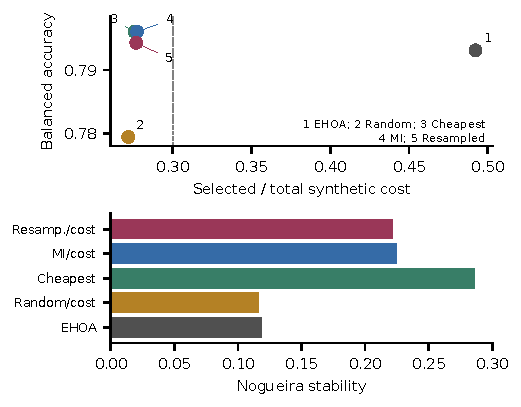
\includegraphics[width=\linewidth]{figures/eligible_comparison.pdf}\par{\footnotesize Figure 1. Fresh ten-dataset means; synthetic cost and descriptive subset stability.\par}\end{minipage}\par
\sect{8  Biomedical case and congress relevance}
Breast Cancer Wisconsin (Diagnostic) has 569 fine-needle-aspirate cases, 212 malignant and 357 benign, with 30 nuclear-image descriptors [15]. Table 7 and Figure 2 show nine fresh masks per method. Counts describe computational selections, not causal biomarkers. Several descriptors share the same image acquisition, so additive synthetic costs cannot be interpreted as biopsy-price savings. Label 0 is malignant and label 1 benign; class-specific recall is explicitly reported.

\par\vspace{3pt}\begin{minipage}{\linewidth}{\footnotesize Table 7. Breast-cancer case: nine fresh runs per method.\par}
{\fontsize{6.8}{8.3}\selectfont\setlength{\tabcolsep}{2pt}\renewcommand{\arraystretch}{1.1}
\begin{tabularx}{\linewidth}{>{\hsize=1.0000\hsize\raggedright\arraybackslash}X>{\hsize=1.0000\hsize\raggedright\arraybackslash}X>{\hsize=1.0000\hsize\raggedright\arraybackslash}X>{\hsize=1.0000\hsize\raggedright\arraybackslash}X>{\hsize=1.0000\hsize\raggedright\arraybackslash}X>{\hsize=1.0000\hsize\raggedright\arraybackslash}X}\toprule
Method & BA & Mal. sens. & Ben. spec. & Cost & Stability\\\midrule
EHOA & 0.9527 & 0.9465 & 0.9589 & 0.5302 & 0.0722\\
Random/cost & 0.9375 & 0.9245 & 0.9505 & 0.2387 & 0.1012\\
Cheapest & 0.9547 & 0.9449 & 0.9645 & 0.2703 & 0.2253\\
MI/cost & 0.9549 & 0.9433 & 0.9664 & 0.2692 & 0.1871\\
Resamp./cost & 0.9503 & 0.9323 & 0.9683 & 0.2781 & 0.1185\\
\bottomrule\end{tabularx}}
\end{minipage}\par\vspace{3pt}
\par\begin{minipage}{\linewidth}\centering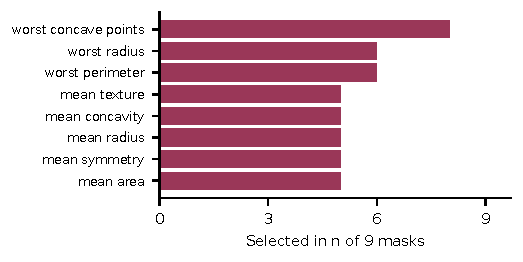
\includegraphics[width=\linewidth]{figures/breast_top_frequencies.pdf}\par{\footnotesize Figure 2. Top eight feature selection counts in nine fresh resampled-repair masks.\par}\end{minipage}\par
The closest official BAIC2026 topic is Artificial Intelligence, Machine Learning and Data Science / Intelligent Disease Diagnosis Systems (baic.um.ac.ir/fa/home/Content/12). The contribution is computational measurement-panel selection; the study is not a clinically validated diagnostic system and makes no cognitive-mechanism claim.

\sect{9  Limitations and reproducibility}
Fold-local utility and selected-dimension SMOTE fix two implementation limitations of the earlier protocol. However, costs remain synthetic; external clinical data and independent verification of subject identity are unavailable. Sensitivity covers three datasets, three seeds and a short search, not all interactions or optimizer settings. MI is marginal; mean-minus-SD has no calibrated coverage. Stability cannot certify clinical relevance. Earlier registration and failure logs cannot be reconstructed by locally freezing this new study.

The local package contains all 774 run records, masks, outer predictions, utility vectors, row indices, candidate-level audit files, full timing and environment versions. Audit checks mask counts, costs, repaired-candidate budgets, train/validation/test separation, group overlap and SMOTE dimensions. New and archived results remain separate. A public repository has not been released; local reproducibility is not public availability.

\sect{10  Conclusion}
The redesigned protocol evaluates the complete training-and-repair pipeline with training-local utility and selected-dimension resampling. All constrained masks are feasible. Interpretation must follow corrected pairwise evidence and compare against feasible simpler repairs. Clinical and monetary claims still require real grouped acquisition costs and independent clinical validation.

\sect{References}
\begin{minipage}{\linewidth}{\fontsize{7}{8.2}\selectfont [1] R. Jagdhuber, M. Lang, A. Stenzl, J. Neuhaus, and J. Rahnenführer, "Cost-Constrained feature selection in binary classification: adaptations for greedy forward selection and genetic algorithms," BMC Bioinformatics, vol. 21, art. 26, 2020. \url{https://doi.org/10.1186/s12859-020-3361-9}\par}\end{minipage}\par
\begin{minipage}{\linewidth}{\fontsize{7}{8.2}\selectfont [2] S. Nogueira, K. Sechidis, and G. Brown, "On the Stability of Feature Selection Algorithms," Journal of Machine Learning Research, vol. 18, no. 174, pp. 1-54, 2018. \url{https://jmlr.org/papers/v18/17-514.html}\par}\end{minipage}\par
\begin{minipage}{\linewidth}{\fontsize{7}{8.2}\selectfont [3] B. Remeseiro and V. Bolon-Canedo, "A review of feature selection methods in medical applications," Computers in Biology and Medicine, vol. 112, art. 103375, 2019. \url{https://doi.org/10.1016/j.compbiomed.2019.103375}\par}\end{minipage}\par
\begin{minipage}{\linewidth}{\fontsize{7}{8.2}\selectfont [4] A. E. Hegazy, M. A. Makhlouf, O. A. M. Salem, and B. Hafiz, "An enhanced Hiking optimization algorithm for accurate and interpretable feature selection in medical data classification," Cluster Computing, vol. 29, art. 244, 2026. \url{https://doi.org/10.1007/s10586-026-05946-9}\par}\end{minipage}\par
\begin{minipage}{\linewidth}{\fontsize{7}{8.2}\selectfont [5] V. Hamer and P. Dupont, "An Importance Weighted Feature Selection Stability Measure," Journal of Machine Learning Research, vol. 22, no. 116, pp. 1-57, 2021. \url{https://jmlr.org/papers/v22/20-366.html}\par}\end{minipage}\par
\begin{minipage}{\linewidth}{\fontsize{7}{8.2}\selectfont [6] T. Klonecki and P. Teisseyre, "Feature selection under budget constraint in medical applications: analysis of penalized empirical risk minimization methods," Applied Intelligence, vol. 53, pp. 29943-29973, 2023. \url{https://doi.org/10.1007/s10489-023-05063-9}\par}\end{minipage}\par
\begin{minipage}{\linewidth}{\fontsize{7}{8.2}\selectfont [7] M. Valancius, M. Lennon, and J. Oliva, "Acquisition Conditioned Oracle for Nongreedy Active Feature Acquisition," Proceedings of the 41st International Conference on Machine Learning, PMLR, vol. 235, pp. 48957-48975, 2024. \url{https://proceedings.mlr.press/v235/valancius24a.html}\par}\end{minipage}\par
\begin{minipage}{\linewidth}{\fontsize{7}{8.2}\selectfont [8] T. Klonecki, P. Teisseyre, and J. Lee, "Cost-Constrained Multi-label Group Feature Selection Using Shadow Features," in Advances in Artificial Intelligence Research, PP-RAI 2025, Lecture Notes in Networks and Systems, vol. 1599, pp. 3-16, Springer, 2026. \url{https://doi.org/10.1007/978-3-032-04197-5_1}\par}\end{minipage}\par
\begin{minipage}{\linewidth}{\fontsize{7}{8.2}\selectfont [9] N. Meinshausen and P. Buhlmann, "Stability selection," Journal of the Royal Statistical Society: Series B, vol. 72, no. 4, pp. 417-473, 2010. \url{https://doi.org/10.1111/j.1467-9868.2010.00740.x}\par}\end{minipage}\par
\begin{minipage}{\linewidth}{\fontsize{7}{8.2}\selectfont [10] R. D. Shah and R. J. Samworth, "Variable selection with error control: another look at stability selection," Journal of the Royal Statistical Society: Series B, vol. 75, no. 1, pp. 55-80, 2013. \url{https://doi.org/10.1111/j.1467-9868.2011.01034.x}\par}\end{minipage}\par
\begin{minipage}{\linewidth}{\fontsize{7}{8.2}\selectfont [11] B. C. Ross, "Mutual Information between Discrete and Continuous Data Sets," PLOS ONE, vol. 9, no. 2, art. e87357, 2014. \url{https://doi.org/10.1371/journal.pone.0087357}\par}\end{minipage}\par
\begin{minipage}{\linewidth}{\fontsize{7}{8.2}\selectfont [12] N. V. Chawla, K. W. Bowyer, L. O. Hall, and W. P. Kegelmeyer, "SMOTE: Synthetic Minority Over-sampling Technique," Journal of Artificial Intelligence Research, vol. 16, pp. 321-357, 2002. \url{https://doi.org/10.1613/jair.953}\par}\end{minipage}\par
\begin{minipage}{\linewidth}{\fontsize{7}{8.2}\selectfont [13] S. Varma and R. Simon, "Bias in error estimation when using cross-validation for model selection," BMC Bioinformatics, vol. 7, art. 91, 2006. \url{https://doi.org/10.1186/1471-2105-7-91}\par}\end{minipage}\par
\begin{minipage}{\linewidth}{\fontsize{7}{8.2}\selectfont [14] J. Demšar, "Statistical Comparisons of Classifiers over Multiple Data Sets," Journal of Machine Learning Research, vol. 7, pp. 1-30, 2006. \url{https://jmlr.org/papers/v7/demsar06a.html}\par}\end{minipage}\par
\begin{minipage}{\linewidth}{\fontsize{7}{8.2}\selectfont [15] W. Wolberg, O. Mangasarian, N. Street, and W. Street, "Breast Cancer Wisconsin (Diagnostic)," UCI Machine Learning Repository, 1993. \url{https://doi.org/10.24432/C5DW2B}\par}\end{minipage}\par
\end{multicols}
\end{document}